\section{User Experience}
We have already dealt with user interface designs in the RASD, where we have shown some mock-ups of the screens of our application.

To maintain reasonable the initial development cost, the PowerEnJoy operators will access to the system through ssh, that can ensure a certain level of security. In the future, a web app for the PowerEnJoy operators will be created.

In this section we will model the user experience of the mobile app, showing how the interface changes with the input of the user and external factors, so we will map the sequence of actions and events with the screens flow.

We will use the class diagram for the user experience modelling. This approach needs some clarification about the used notation, so below we are going to explain the meaning of the symbols used:

\begin{description}
\item[Directed arrow:] It defines a transition from a particular user interface element to another. It may be due to two possible cause:
	\begin{description}
	\item[User input:] This type of transition is triggered by the invoking of a particular method \textit{function()} in the source interface element.
	The name of the user input transaction is the same of the function that was invoked by the user. Sometimes the method can rise an error, so in these cases the name of the transaction is followed by "ok" if the outcome of the function is positive or by "error" if it is negative. 
	\item[Event:] This type of transition is triggered by an event that can be generated by the client itself or by a message sent  by the server to the client. This transaction is identified by the "event" at the end of the name.
	\end{description} 
\item[Class symbol:] It determines a specific user interface element among \textit{Screen}, \textit{Input form}, \textit{Element}, \textit{Pop-up}\ and \textit{Frame}
or a specific event (stereotype \textit{event}). In both cases the type of element is specified in the stereotype of the class symbol. 
\item[Composition symbol:] Means that a specific user interface element is contained in another. Typically is used when a form or a list of elements is contained in a particular screen. It can be also used to say that a generical user interface element displays some info.
\end{description}

It is important to underline that, in order to maintain readability, only the main elements are shown in the following diagram.

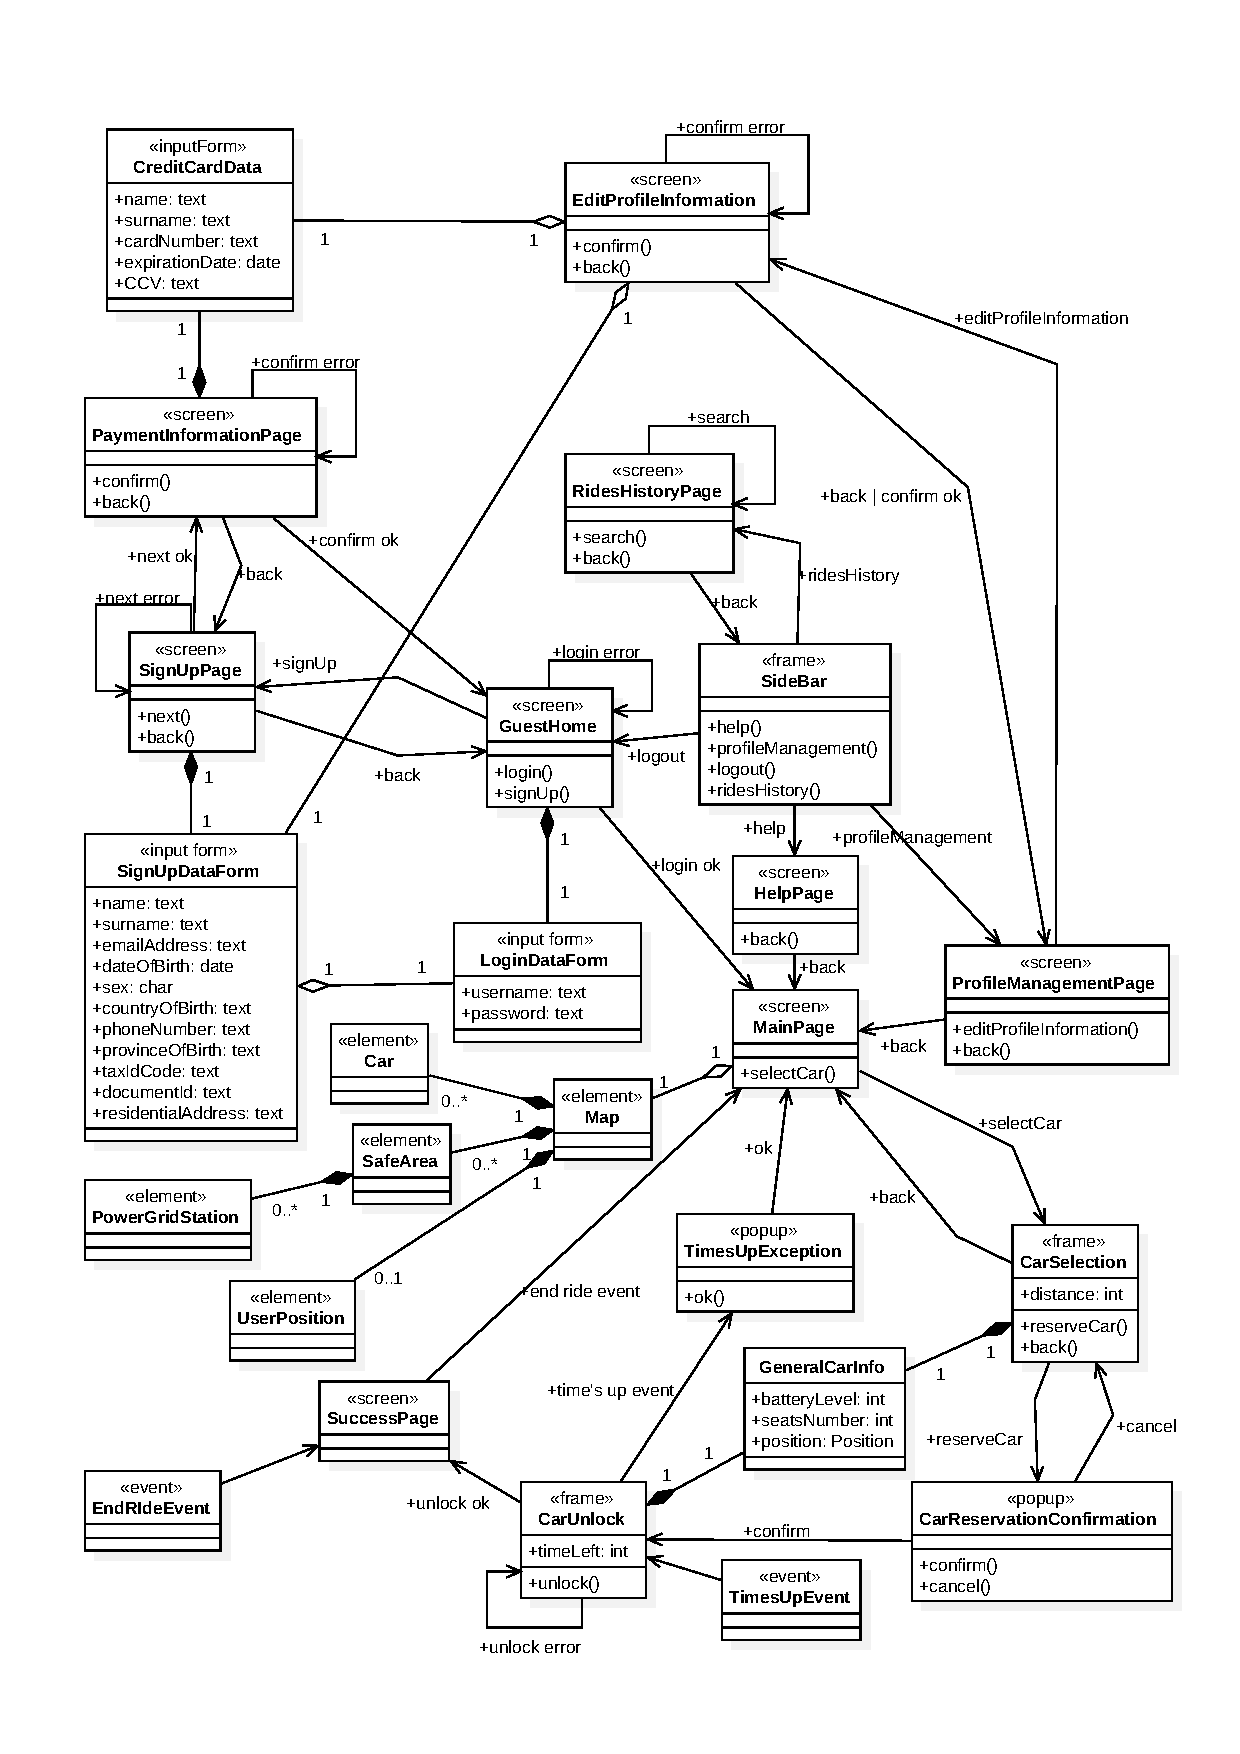
\includepdf{ui_design/user_experience.pdf}
